\chapter{Text\INDEV}

Sometimes you can spot data leakage by simply opening a file with an
ordinary utility, as we did in the last chapter when we used Apple's
Preview application to read geolocation data hidden inside a JPEG. 

Other times the leakage may be less obvious.  The software developers
know that the information is present but don't think that it's
relevant, and people who are in a position to know that the leakage is
relevant don't have the technical ability to determine that it's
present.

This chapter explains how text is stored in a
computer. \secref{sec:letters} discusses
how ASCII, code pages, and Unicode are represented in the computer. 

In order to understand what the hex dump and extracted strings
actually mean, we'll need to see how numbers 
numbers (\secref{sec:numbers}) and letters (\secref{sec:letters}) are 
digitally stored.  Much of this chapter is similar to
what might be covered at the start of a course on computer
architecture. But whereas an architecture course is primarily
concerned with computation and data in motion, this chapter is
concerned with understanding data at rest.

This chapter starts with instructions for creating a file that has hidden information
(\secref{sec:make-pdf}). We'll save the file in two ways, as a Rich
Text file (RTF) and as a Portable Document Format (PDF) file. Then
we'll look at the data the file contains using a variety of
techniques, including the raw bytes, a a \emph{hex dump}
(\secref{sec:hex-dumps}), and by extracting the printable strings
(\secref{sec:strings}). 


\section{From Bits to Numbers}\label{sec:numbers}
The \emph{bit} is the fundamental unit of storage on digital computers. Bits
have two states. Typically we call these |0| and |1|. (The word
\emph{bit} is a contraction of the words \emph{binary digit}.) 
An ordered group of 4 bits is called a \emph{nibble}. Each bit can be
a |0| or a |1|, creating 16 possible different values. (Note
that $2^4=16$.) It is conventional to use the digits 0 through 9 to
number the first 10 possible nibble values, and use the letters A
through F to number the next six, as shown in \figref{nibble}. By
convention computer users call this notation \emph{hexadecimal},
although it's also called Base 16.

\begin{figure}
\begin{tabular}{>{\tt}c>{\tt}cc>{\tt}cl}
\textrm{binary} & \textrm{octal} & decimal & \textrm{hexadecimal} & english \\
\hline
0000b & 000 & 0 & 0h & zero \\
0001b & 001 & 1 & 1h & one \\
0010b & 002 & 2 & 2h & two \\
0011b & 003 & 3 & 3h & three \\
0100b & 004 & 4 & 4h & four \\
0101b & 005 & 5 & 5h & five \\
0110b & 006 & 6 & 6h & six \\
0111b & 007 & 7 & 7h & seven \\
1000b & 010 & 8 & 8h & eight \\
1001b & 011 & 9 & 9h & nine \\
1010b & 012 & 10& Ah & ten \\
1011b & 013 & 11& Bh & eleven \\
1100b & 014 & 12& Ch & twelve \\
1101b & 015 & 13& Dh & thirteen \\
1110b & 016 & 14& Eh & fourteen \\
1111b & 017 & 15& Fh & fifteen \\
\hline
\end{tabular}
\caption{A nibble is an ordered collection of 4 bits. Each bit can be
  a 0 or 1, so a nibble has $2^4=16$ possible values. This table shows
  the values of a nibble represented in binary, octal, decimal hexadecimal and English.}\label{nibble}
\end{figure}

Modern computers operate on groups of 8 bits at a time, which we call
\emph{bytes}. There are $2^8=256$ possible byte values. This book will
normally treat bytes as unsigned integers in the range 0 to 255, but
that is just a convention; Java treats bytes as signed integers in the
range $-128$ to 127. It's also common to use present the value of a
byte in hexadecimal notation, with the range |00| through |FF|. 

There are many ways to combine bytes to store more than 256
values. Virtually all modern systems allow for single math operations on 2
bytes (a 16-bit word), 4 bytes (a 32-bit long), or 8 bytes (a 64-bit
double long). These values can be unsigned or signed. Fixed numbers of
bytes can also be used to hold floating point values. Finally, many
computer languages and libraries can represent numbers with variable
length strings of bytes for arbitrary precision.

\section{Text, ASCII, Code Pages and Unicode}\label{sec:letters}

To store text in a computer's memory it is necessary to convert the
text into a series of numbers. This conversion is performed using a 
\emph{code} or a \emph{mapping}. One of the most common codes used in
the past was ASCII, the American Standard Code for Information
Interchange. ASCII uses just 7 bits (the 8th was reserved for error
checking) and has the ability to represent letters, numbers, 32
symbols, and a number of ``control'' characters used for
signaling. ASCII was adopted as a US standard in 1972 and remains in
use to this day.

With ASCII, each character appears in alphabetical or numerical ASCII
was designed to make it relatively simple to process text inside a
computer. A space is coded with 64 (|40h|), the capital letter ``A''
is coded with 65 (|41h|), ``B'' is a 66 (|42h|), and so on. To get the
codes for lower case letters simply add 32, so the lower case ``a'' is
96 (|61h|) and ``b'' is 97 (|62h|).  A chart from a 1972 printer
manual showing the relationship between the binary codes, control
characters, letters and symbols appears in \figref{ch-what/ascii}.


\sgraphic{ch-what/ascii}{An ASCII chart from a 1972 printer manual,
  courtesy of Wikipedia. The hexadecimal code for each letter is
  simply the column label followed by the row, although the row must
  be converted from decimal to hex. For example, the ``A'' is \texttt{4a}
  while the ``M'' is \texttt{4d}.}

For example, the sequence of letters ``Hello World!'' would be
represented by the ASCII sequence |48 65 6c 6c 6f 20 57 6f 72 6c 64 21|.

\subsection{Hex Dumps}\label{sec:hex-dumps}
A common way to visualize binary data is to format it as a series of
text lines, with each line containing a series of hexadecimal values (one
for each binary byte). Such displays are called \emph{hex
  dumps}.

There are many different programs that produce hex dumps, and each
program formats its output in a slight different manner. Fortunately
there is enough commonality that you can usually look at a hex dump
and figure it out. Most dumps will have a column on the left that
displays the offset in bytes from the beginning of the data, and a
column on the right that shows the ASCII representation of each
byte. Dumps are typically formatted such that each line represents 32
or 64 bytes of data.

Below is a hex dump for the 28-byte string 
|Hello World!\r\nHello World!\r\n| created with the Unix \emph{xxd}
program. (Notice that the hexadecimal numbers \emph{do not} have a
``h'' suffix.)

\begin{Verbatim}
0000000: 4865 6c6c 6f20 576f 726c 6421 0d0a 4865  Hello World!..He
0000010: 6c6c 6f20 576f 726c 6421 0d0a            llo World!..
\end{Verbatim}

In a hex dump the period (``.'') is used to represent characters that
have no printable ASCII equivalent. In the example above the period is
used for the control characters carriage return (|0d|) and line feed (|0a|).

One quick way to analyze unfamiliar programs or data  is to look for printable
strings. Long strings can be guideposts: the longer the string, the
less likely it is to be repeated by chance in another program or data
file. Another quality of strings is that they are invariably authored
by another person. 

With large blocks of data it can be hard to find the printable
strings. Consider the file (random48.bin). This file contains the word ``Privacy'', but it can be hard to
find: 

\begin{code}
$ (@ \hl{xxd random48.bin} @)
0000000: fdf8 7c33 a153 0516 cc72 84fc 0050 7269  ..|3.S...r...Pri
0000010: 7661 6379 1437 ed4d e84b 0280 a74f e64b  vacy.7.M.K...O.K
0000020: 4695 6a66 9549 2cc9 4109 83c1 3e96 766b  F.jf.I,.A...>.vk
\end{code}
%$


Instead of manually scanning for strings, you can use the Unix
\emph{strings} program to find ASCII strings and print them on the
computer's output. 

\begin{code}
$ (@ \hl{strings random48.bin} @)
Privacy
\end{code} 
%$

The \emph{strings} program works by looking for sequences of printable
ASCII characters surrounded by non-printable characters. By default,
the program will print any sequence of printable bytes longer than 4
characters. \emph{strings} is frequently used for reverse engineering software
because it frequently displays the messages that a program might
print. Unfortunately, there are many ways to hide text so that the \emph{strings}
program will not show it, so the fact that a string isn't shown does
not mean that it is not present. 

Any transformation to the string that replaces ASCII characters with
non-ASCII characters will render the string invisible to the
\emph{strings} command. These transformations include:

\begin{itemize}
\item Encrypting the string with any encryption algorithm.
\item Compressing the string with any compression algorithm.
\item Using (XOR 255) to invert the string's bits.
\item Turning the string into a picture
\end{itemize}

\section{Latin-1 (ISO 8859-1)}

\section{Unicode}

Unicode is the international standard used by all modern computer
systems to define a mapping between information stored inside a
computer and the letters, digits and symbols that are displayed on
screens or printed on paper. Unicode is a proper superset of
ASCII. Thus, a Unicode decimal 65
stored in a computer's memory is displayed as a capital letter
``A'', while a decimal 97 is a lower case ``a''.

Unlike ASCII, Unicode has hundreds of thousands of characters. The
goal is that any printable character in any human language (live or
dead) should be displayable with Unicode. 

Unicode characters are described by their ``code point,'' which
written as a ``U+'' followed by a four or five digit hexadecimal
number. Every Unicode
character also has a unique name in English that's
written with uppercase letters---for example, \pounds\xspace is POUND SIGN. Every
Unicode character also has a unique numeric code, which Unicode calls
a "code point," that's written with a U+ followed by a four or five
character hex code. One of the most common Unicode characters that
will not fit in 8-bits is the EURO SIGN (\euro~or U+20AC). Code points over 65,536 are
particularly troublesome. Fortunately they are mostly used for unusual
Chinese characters and letters in ancient scripts, such as AEGEAN
NUMBER SIX THOUSAND (U+10127).

As the preceding paragraph demonstrates, Unicode is dramatically more
complex than the 7-bit ASCII and the so-called "Latin1" (actually ISO
8859-1) systems that it replaces. But Unicode brings more complexity
than an expanded character set. For example, Unicode accented
characters can be represented with a single code point (for example
LATIN SMALL LETTER E WITH ACUTE, \'{e} or U+00E9), or with a so-called
combining character followed by another character (for example,
Unicode character COMBINING ACUTE ACCENT (U+0301) followed by a
Unicode character LATIN SMALL LETTER E (U+0065).

The  Unicode standard also has rules for displaying and correctly
processing writing systems that go right-to-left such as Arabic,
Hebrew and Dhivehi. Before Unicode it was a complex task to build
computer systems that could properly display text that way, let alone
intermix right-to-left with left-to-right. Unicode's support for
bidirectional text largely eliminates these problems, making it
possible to freely use Arabic words like
\raisebox{-4pt}{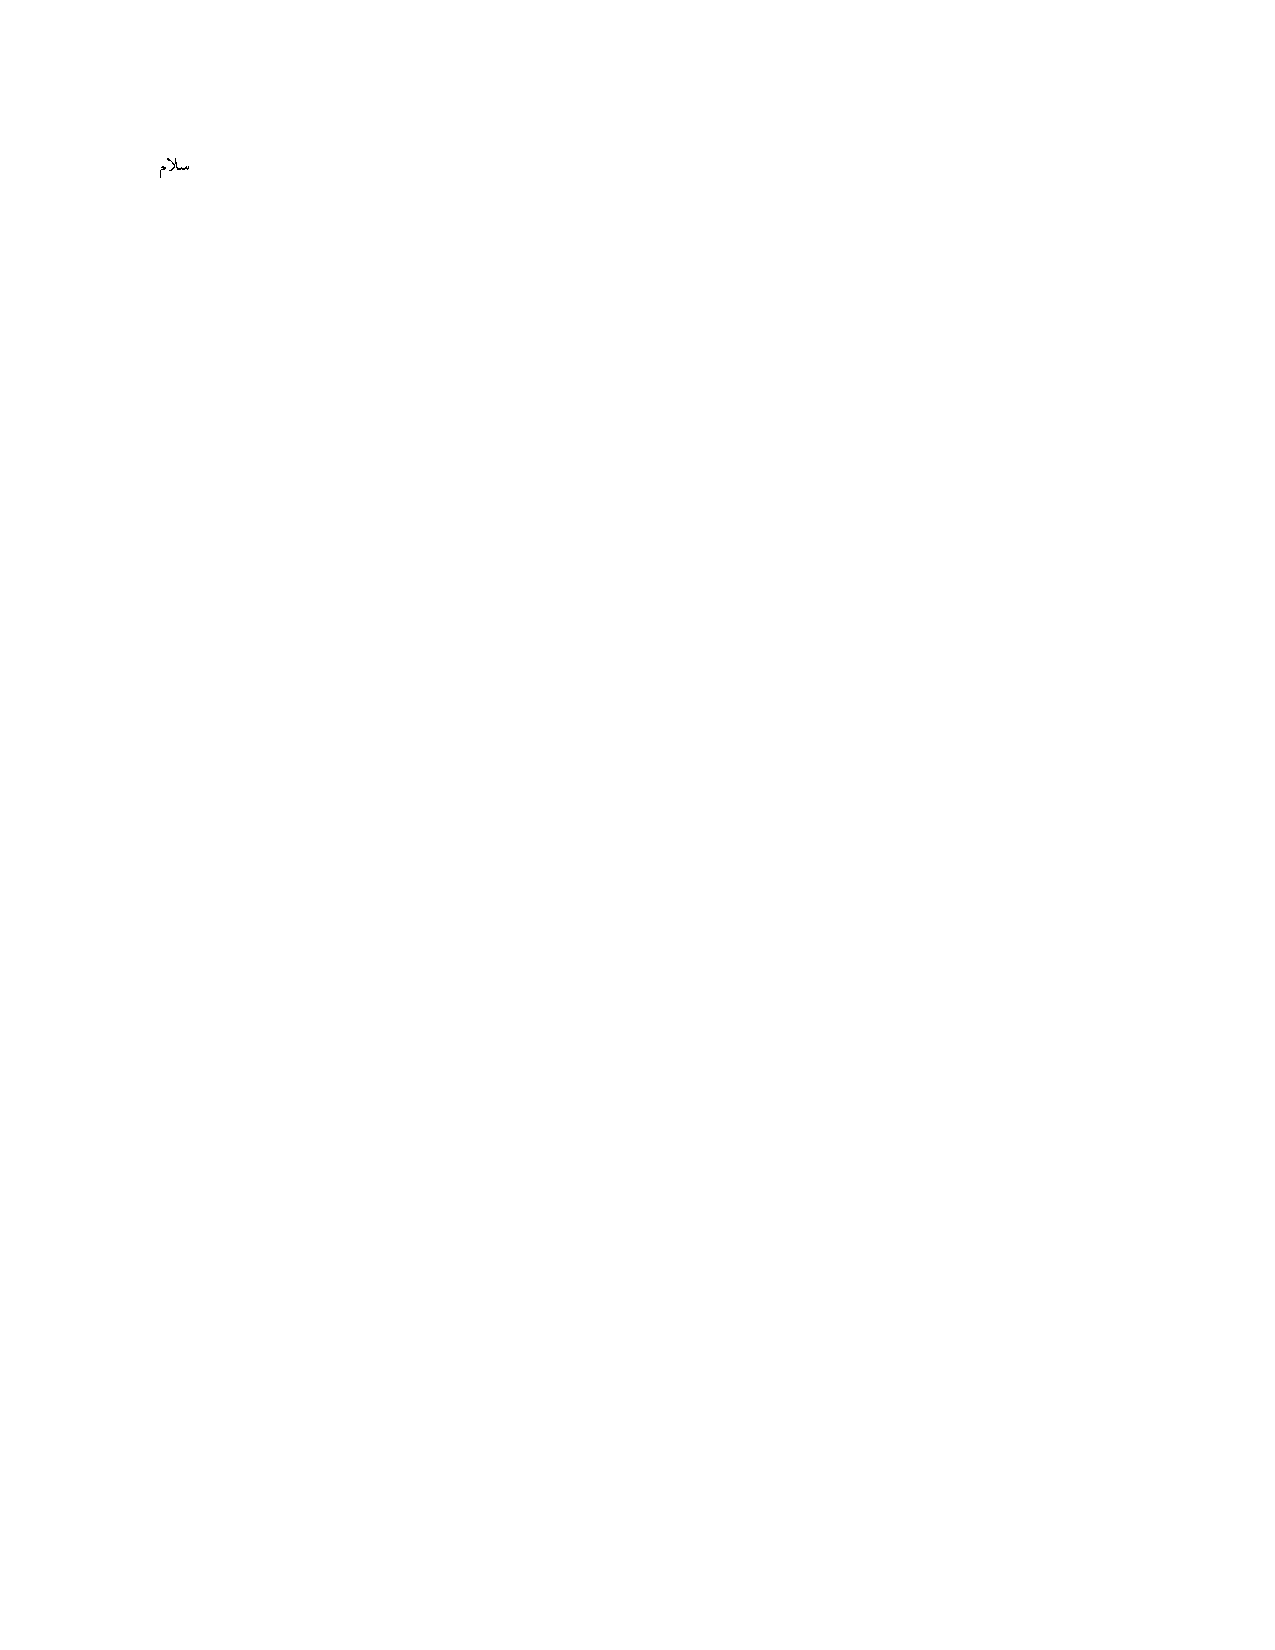
\includegraphics{ch-what/saalem}}  in English text. 

\subsection{Code Points and Characters}

Like ASCII and ISO8859-1, at its most fundamental level the Unicode
standard defines a mapping between code points and print
characters. The big difference is quantity: Unicode's most recent
version, Unicode 6.0, defines more than 109,000 printable objects.

Most of the code points map to characters, which the standard  calls
``graphemes.'' A grapheme is a unit of written language such as the
letter "a" (U+0061), the number "1" (U+0031) or the Kanji for man
``\raisebox{-4pt}{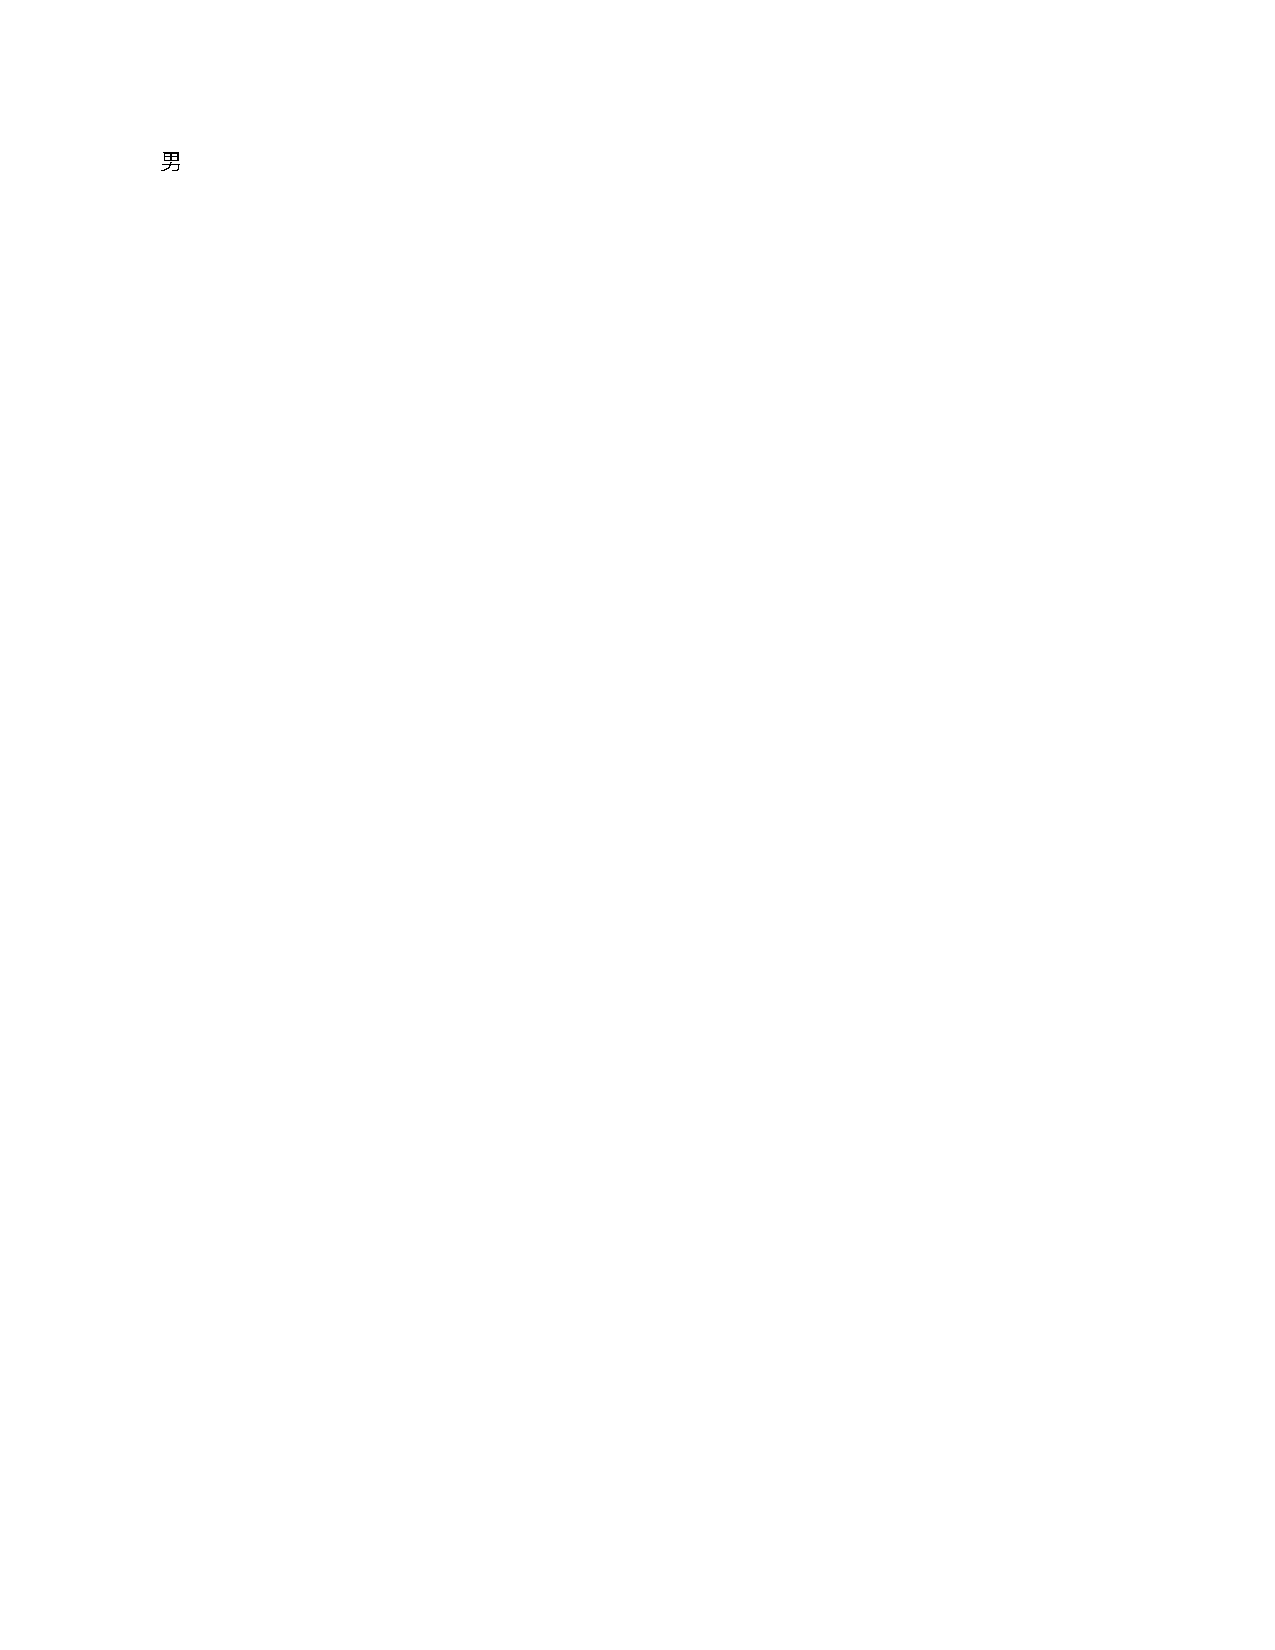
\includegraphics{ch-what/man}}'' (U+7537). Most graphemes are
displayed as a single glyph, which is the smallest printable unit of a
written language.  

Unicode terminology is precise and frequently misused: the confusion
is frequently reflected by errors in Unicode implementations. For
example, a grapheme (such as the lower case ``a'') can be displayed by
two distinct glyphs (in the case of an ``a'', one of the glyphs looks
like a circle with an attached vertical line on the left, while the
other looks like a slightly smaller circle with a hook on the top and
a tail in the lower-right quadrant).  Both glyphs are represented by
the same code point. But some glyphs can represent two
characters---for example, some typesetting programs will typeset the
letter ``f'' (U+0066) followed by the letter ``i'' (U+0069) as an ``fi''
ligature (U+FB01), which has a single distinct code
point. Typesetting programs do not expect to see a U+FB01 in their
input file, for the simple reason that people don't type
ligatures. It's the typesetting program that replaces the U+0066
followed by the U+0069 with a U+FB01, adjusting spacing as appropriate
for a specific font.

Arabic is even more complex. Arabic graphemes are written with
different glyphs depending if the grapheme appears at the beginning,
end, or in the middle of a word. In the case of Arabic, most of the
letters actually have four code points assigned: one that represent
the abstract character and three ``presentation'' code points that
represent each printable form. The abstract character might be used
inside a word processor document, while the presentation forms are
used in files that are rendered for display---for example, in a PDF
file. Microsoft's implementation of Arabic is different for various
versions of Word, Excel, and Powerpoint on the Mac and PC. As a
result, a file containing Arabic that looks beautiful on one platform
can look poor on another. Web-based text editors can have similar problems when used to edit Arabic documents.

Every modern programming language supports Unicode, but frequently
with types and classes that are different from those taught in
school. For example, C and C++ programmers should use the |wchar_t| type
to hold a Unicode character (or any other printable character, for
that matter), defined in the |<wchar.h>| header. Unicode strings are
best represented in C++ with the STL |std::wstring| class defined in
the <string> header. The Python3 |string| type can hold 0, 1 or
multiple Unicode characters; there is no separate type for an
individual character. If you are still using Python2, the |string|
class holds ASCII and you need to specify |unicode| (or |u""|) to
create a Unicode character or string. In Java the |char| primitive
type and the |Character| class hold Unicode code points, but only
those characters with values less than U+FFFF. These code points are
said to reside in the Basic Multilingual Plane (see next section). Code points that require more than
16 bits are represented by a pair of code points, as we will see
below.

\subsection{Expanding The Basic Multilingual Plane}

Before Unicode many manufacturers developed their own propriety
systems for representing Chinese or Japanese using 16-bit characters,
sometimes called ``wide'' characters. One of the original goals of
Unicode was thus something called ``Han Unification''---that is, for
manufacturers to be able to use the same code points to denote
ideographs that were the same both languages. The designers were able
to get nearly all of the characters they needed to fit into the 65,536
code points allowed by a 16-bit word. This 2-byte encoding was called
UCS-2, for Universal Character Set, 2-byte encoding.

Unfortunately, 65,536 characters were not sufficient to represent all
of the Chinese logograms, let alone characters for all of the world's
ancient languages. The first 64Ki characters were deemed to belong to
a ``code plane'' and 16 more were created. Code Plane 0 is the Basic
Multilingual Plane and covers Unicode characters U+0000 through U+FFFF
(although U+FFFF is explicitly not a valid Unicode character). Code
Plane 1 is mostly used for additional symbols, Plane 2 for additional
ideographs, Pane 14 for special purpose, and Planes 15 and 16 for
"private use." Planes 3-13 are currently unassigned. With so much room
to grow, it is highly unlikely that Unicode will ever need to be
expanded beyond the 17 code planes (\tabref{code-planes}).

\begin{table}
\begin{tabular}{lll}
	Plane 0:    &   0000- FFFF &   Basic  Multilingual Plane (BMP)\\
	Plane 1:    &  10000-1FFFF &   Supplementary Multilingual Plane (SMP)\\
	Plane 2:    &  20000-2FFFF &   Supplementary Ideographic Plane (SIP)\\
	Planes 3-13:&  30000-DFFFF &   Unassigned\\
	Plane 14:   &  E0000-EFFFF &   Supplementary Special Purpose Plane (SSP)\\
	Planes 15-16:& F0000-10FFFF&   Supplementary Private Use Area (S PUA A/B)\\
\end{tabular}
\caption{Unicode code planes}\label{code-planes}
\end{table}

The assignment of code planes is arbitrary, but there is some
sensibility in the allocation. Plane 0 was first. The extension
mechanism that the standards body adopted allows an additional 4 bits
to be optionally specified; Plane 1 has all of those additional bits
set to 0, Plane 16 has them all set to '1', and Plane 0 is marked by
the absence of those optional bits. Planes 1 and 2 are really the only
additional planes that were mapped out by the Committee; the top two
Planes were reserved for private use. Because Planes 3-13 are
unassigned, they can be trapped as errors.

Many systems (like Java) were designed to be Unicode-aware when
Unicode only had 16-bit characters.  Unicode 2.0's creators thought
that they would not be able to get programmers to change their systems
to use 32-bit characters---especially when most of the bits would
always be 0. Instead, a coding scheme was developed that allowed pairs
of 16-bit code points the BMP to represent characters with code points
greater than 65,535. These pairs are called ``surrogates.''

Consider the SQUARED FREE (U+1F193). This code point can be
represented with 4-bytes using a sequence of four hex characters, 00
01 F1 93. But the code point can also be represented with a pair of
Unicode characters called "surrogates." The 18 bits of code points
outside the BMP to be divided into two halves, with 9 bits encoded by
a first surrogate in the range D800-DBFF and 9 bits encoded using a
second surrogate in the range DC00-DFFF. In the case of U+1F193, the
two surrogates are U+D83C and U+DD93. Java always uses surrogates to
represent characters outside the BMP.

Python can be compiled to use either 16-bit or 32-bit Unicode code
points for its internal representation. If sys.maxunicode is 65535,
then your Python interpreter is using surrogates internally to
represent characters outside the BMP; if sys.maxunicode is 1114111,
the Python interpreter can represent all Unicode characters without
surrogates internally. Python uses the |\u| escape to specify code
points in the BMP and |\U| to specify 32-bit code points (even though
only 21 bits are considered.)

The way C and C++ handle characters outside the BMP depends on the
platform.  Under GCC/G++ 4.2 on Mac and Linux systems, |wchar_t| is a
32-bit value, allowing Unicode characters outside the BMP to be stored
directly. But compile a program with Microsoft's Visual Studio or the
mingw cross-compiler, and |wchar_t| is a 16-bit quantity. Frankly it's
hard to notice the difference, provided you always allocate memory in
|sizeof(wchar_t)| chunks and never depend on the size of a Unicode
string being related in any way to the number of characters that it
contains.  

All of this is less complicated in practice if you use a high-quality
Unicode implementation that hides these details and write clean C++
code. 


\subsection{Encoding and Decoding}

So far this article has been discussing Unicode in the abstract and has avoided the messy issue of reading and writing Unicode data. The issue is messy because modern computer systems read and write data in 8-bit bytes, but Unicode needs a minimum of 16 bits to represent characters in the BMP and 21 bits[10] to represent all possible code points (or two 16 bit pairs if surrogates are used).

Early Unicode implementations, like the one in Microsoft Windows, took the rather straightforward approach of storing everything as 16-bit UCS-2 characters. When Microsoft needed to store Unicode on disk---for example, in a file name---it simply wrote the bytes in the same order that they were stored in memory. This process of transforming abstract code points to a specific set of 8-bit codes stored in a file or sent down a wire is called "encoding."

Clearly, there are two ways for a 16-bit code point such as U+0061 to be encoded: as a 61 followed by a 00 (called "little endian," because the little end comes first), or as a 00 followed by a 61 ("big endian.") Rather than mandating that Unicode be encoded in one way or the other, Unicode supports both byte orders. UTF-16LE (UCS Translation Format--16 bit Little Endian) is what Windows uses.

For example, the FAT32 file system store both legacy ISO8859-1 8.3 filenames and UTF-16LE filenames that can be up to 255 characters long. NTFS file systems only store UTF-16LE filenames. This means that the filename README.TXT is stored as the UTF-16LE sequence 52 00 45 00 41 00 44 00 4d 00 45 00 2e 00 54 00 58 00 54 00. Most of the Windows API functions that operate on files have two versions---one that takes ISO8859-1 names terminated with a 00, and one that takes UTF-16LE "wide" names terminated with a 00 00. For creating files these are the CreateFile() and CreateFileW() functions. 

Similar to the 2-byte encodings, Unicode also supports 4-byte encodings UTF-32LE and UTF-32BE. With the UTF-32LE encoding the string "READ" would encode as 52 00 00 00 45 00 00 00 41 00 00 00 44 00 00 00. Such encodings are rarely used outside of a computer's memory because of the storage cost.

Unicode provides a special code called the Byte Order Mark (BOM, U+FEFF) that can be stored inside a file and used to unambiguously indicate whether the file is encoded as UTF-16LE, UTF-16BE, UTF-32LE, UTF-32BE or using the variable-length UTF-8 code (see below). The BOM approach works because the byte-swapped character U+FFEE is defined to be an invalid code point. Thus, by looking at the first 2 or 4 bytes of a  file, it is possible to determine the encoding (\tabref{unicode-bom}).

\begin{table}
\begin{tabular}{ll}
	Initial Bytes		&Encoding \\ 
\hline
	00 00 FE FF &       UTF-32, big-endian\\
	FF FE 00 00 &       UTF-32, little-endian\\
	FE FF       &       UTF-16, big-endian\\
	FF FE       &      UTF-16, little-endian\\
	EF BB BF    &      UTF-8 (see below)\\
\end{tabular}
\caption{Unicode Byte Order Mark Signatures}\label{unicode-bom}
\end{table}

From the above examples it may seem that a program can trivially convert between Unicode to ASCII by simply removing or inserting alternating NULL characters. You should never do this!!!  This simplistic approach will fail if the Unicode string contains anything other than code points in the range U+0001 through U+00FF. Instead, programs should explicitly encode Unicode strings from an abstract internal representation when strings are transformed for operating system APIs, sent over a network connection or persisted into a file. Likewise, when data is read from an external source it should be decoded from the wire format into the program's internal representation.


\subsection{UTF-8}

UTF-8 is a system for encoding Unicode code points using a
variable-length sequence of 8-bit characters. UTF-8 has the property
that 7-bit ASCII characters are directly coded as a single UTF-8 byte,
making UTF-8 upwards compatible from ASCII. Characters in the range
U+0080 through U+07FF are coded as two bytes; the remaining characters
in the BMP are coded as three bytes; characters outside the BMP are
coded as four (see Table 3). 

The UTF-8 scheme makes it possible to identify the start of a UTF-8 character from within a randomly chosen block of UTF-8 encoded bytes: if the most significant bit is a 0, then the character is a 7-bit UTF-8 character. If the high bits are "10" then it is a continuation character: move forward or backwards until a byte is found that begins "0" or that begins "11". The number of "1"s in a row indicate the number of bytes in the sequence.

As the table makes clear, UTF-8 is great for Americans, since documents coded in UTF-8 are the same size as documents coded in ASCII. For Europeans the advantage of UTF-8 is that all of their accented characters can be displayed, with only the non-ASCII characters taking up two bytes. For the Chinese UTF-8 is not so good, as it results in a 50\% expansion for most text.


\begin{table}
\begin{tabular}{llllll}
    Bits &Code Point Range  &  Byte 1 &    Byte 2&    Bytes 3&    Byte 4\\
    7    &U+0000  -- U+007F  & 0xxxxxxx&\\
    11   &U+0080  -- U+07FF  & 110xxxxx&   10xxxxxx&\\
    16   &U+0800  -- U+FFFF  & 1110xxxx&   10xxxxxx&  10xxxxxx&\\
    21   &U+10000 -- U+1FFFFF& 11110xxx&   10xxxxxx&  10xxxxxx&  10xxxxxx\\
\end{tabular}
\caption{UTF-8 Encoding}
\end{table}

One of the primary advantages of UTF-8 is that the NULL character is never used. This means that the POSIX APIs can be used more-or-less transparently with UTF-8 encoded Unicode. The confusion here, however, is that UTF-8 is not Unicode---it is a Unicode encoding. Keeping your program's internal data encoded in UTF-8 is fine as long as the strings are viewed atomically and no string operations such as comparison, search, case change, or splitting even needs to be performed by the program. All of these operations require decoding the UTF-8 sequences into Unicode characters and then re-encoding the Unicode characters back to UTF-8.


\section{Searching for private information}


\section{Creating a File with ``Hidden'' text}\label{sec:make-pdf}

\figref{ch-what/textedit_hidden_1} shows how to create a simple file that
contains hidden data using Apple's TextEdit application.\footnote{The
  same set of steps will work with Libre Office or Microsoft Word. We
  use TextEdit here because the resulting RTF and PDF files are the
  simplest.}
 Start by
opening the TextEdit application, type the text, select the word ``Hidden'' and
change the background (highlight) color of the text from ``none'' to
``black.'' (The text background control is the box that looks like this:
\includegraphics[height=1.5ex]{ch-what/textedit_highlight_control}).

Save two copies of the file, one in the Rich Text Format (RTF) in file
a called |hidden.rtf|, the second as an Adobe Portable Document Format
(PDF) file in a file named |hidden.pdf|. (You can use
the same approach with other word processors, but the resulting PDF
file is typically more complicated) 


\bifigure{ch-what/textedit_hidden_1}{ch-what/textedit_hidden_2}{Constructing a PDF with
  hidden text by selecting the text in a word processor (left) and
  then setting the highlight color to black (right).}

The file |hidden.rtf| is seven lines long and has just 297 bytes; that
file's contents appear in \lstref{hidden.rtf}. The file |hidden.pdf|, in
contrast, is 8304 bytes long. If the file's contents were printed here
they would look like a confusing jumble of letters, numbers, and
obscure symbols that would fill four pages. Such jumbled output is 
sometimes referred to as \emph{garbage}, and more properly termed
\emph{binary data} to distinguish it from the printable text that
makes up |hidden.rtf|. 

\sgraphic{ch-what/textedit_hidden-more}{The file {\tt hidden.pdf} viewed with the program \emph{less} running inside the Macintosh Terminal program.}

\lstinputlisting[caption=hidden.rtf,label=hidden.rtf]{ch-what/textedit_hidden.rtf}

\subsection{Viewing a text file}
\subsection{Viewing a binary file}

Attempt to view the file |hidden.pdf| with the
Unix program \emph{less} and you'll be warned:

\begin{code}
$ (@ more hidden.pdf @)
"hidden.pdf" may be a binary file. See it anyway?
\end{code}
%$

Type ``y'' and you'll see results similar to
\figref{ch-what/textedit_hidden-more}. The rest of this chapter explains what
this display means.

\section{Magic Numbers}

\section{Encoding Binary Data}

BASE16, BASE64 and BASE85

\subsection{Legacy Encoding Methods}
uuencode

binhex


\section{Exercises}
* Convert numbers to different bases

* Look for private information with strings in files





